\section{Dateiquelle w�hlen/Spalten zuordnen}
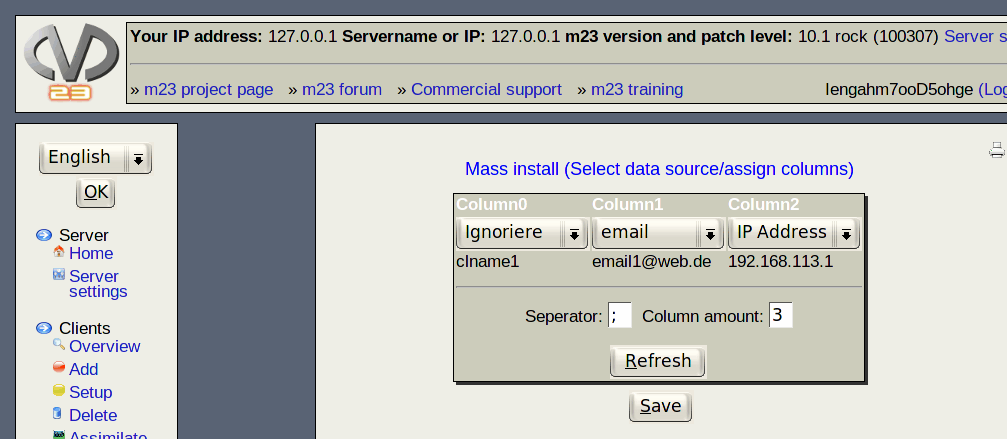
\includegraphics[scale=0.33]{/mdk/doc/manual/screenshots/de/mi_step2.png} \\
Dieser Dialog ist in zwei Schritte aufgeteilt:\\
\begin{itemize}
\item Datei ausw�hlen und hochladen\\
\item Den Feldern in der Datei die Client-Eigenschaften zuweisen\\
\end{itemize}
\subsection{Datei ausw�hlen und hochladen}
W�hlen Sie eine Datei �ber den Dialog aus und klicken Sie danach auf \textit{"Hochladen"}.\\
Die Datei mu� speziell aufgebaut sein, damit m23 die Werte erkennen kann. Pro Zeile werden die Eigenschaftswerte f�r je einen Client spezifiziert. Die einzelnen Eigenschaften werden durch ein Trennzeichen (hier ";") getrennt:\\
\begin{verbatim}
Eigenschaft1;Eigenschaft2;Eigenschaft3;...
\end{verbatim}
An Stelle eines Semikolons kann jede Kombination von bis zu 4 Zeichen verwendet werden. Die Reihenfolge der Eigenschaften mu� in allen Zeilen gleich sein.\\
\subsection{Hinweis}
Neben der grundlegenden Bedingung, da� die in der Datei abgelegten Werte zu den Eigenschaften passen m�ssen, gelten f�r folgende Eigenschaften die zus�tzlichen Bedingungen:\\
\begin{itemize}
\item \textbf{Anmeldungsdaten lokal auf dem Client speichern.}: Wert "yes" aktiviert diese Option, jeder andere Wert deaktiviert sie.\\
\item \textbf{LDAP}: Es sind 3 verschiedene Werte zul�ssig:\\
\begin{itemize}
\item "none": LDAP nicht benutzen\\
\item "read": Anmeldungsdaten vom gew�hlten LDAP-Server lesen.\\
\item "write": Anmeldungsdaten in den LDAP-Server speichern.\\
\end{itemize}
\end{itemize}
\subsection{Den Feldern in der Datei die Client-Eigenschaften zuweisen}
Nachdem Sie eine Datei hochgeladen haben, k�nnen Sie den einzelnen Feldern in der Datei die Eigenschaftsnamen der Clients zuweisen.\\
\subsection{Gehen Sie hierzu wie folgt vor}
\begin{enumerate}
\item Geben Sie das Trennzeichen in das vorgesehene Feld ein und passen Sie ggf. die Spaltenanzahl an.\\
\item Klicken Sie auf \textit{"Aktualisieren"}.\\
\item Weisen Sie nun den Feldern aus der Datenbankdatei die Eigenschaftsnamen aus den Listen zu.\\
\item Schlie�en Sie Ihre Auswahl mit einem Klick auf \textit{"Speichern"} ab.\\
\end{enumerate}
